% Mapa de memoria del módulo central (ONX3248G035, ESP32-S3).
% Se compila por separado: pdflatex mapa_memoria.tex -> mapa_memoria.pdf
\documentclass[tikz,border=4pt]{standalone}
\usepackage[utf8]{inputenc}
\usepackage[T1]{fontenc}
\usepackage{cmbright}
\usepackage{enumitem}
\usetikzlibrary{calc}

\definecolor{cflash}{RGB}{214,120,20}
\definecolor{csram}{RGB}{31,94,168}
\definecolor{cpsram}{RGB}{130,50,140}
\definecolor{csd}{RGB}{30,120,60}

\newcommand{\lista}[1]{%
  \begin{itemize}[leftmargin=10pt, itemsep=1pt, topsep=0pt, parsep=0pt, label=\textbullet]#1\end{itemize}}

% \bloque{nombre}{posición}{color}{título}{propiedades}{alto del encabezado}{alto del cuerpo}{contenido}
\newcommand{\bloque}[8]{%
  \node[anchor=north west, minimum width=8.2cm, text width=7.8cm, align=center,
        minimum height=#6, fill=#3!28, text=black, rounded corners=3pt, inner sep=5pt]
        (#1h) at (#2) {\large\textbf{#4}\\[2pt]{\normalsize #5}};
  \node[anchor=north west, inner sep=6pt, fill=#3!6, draw=#3, line width=0.8pt,
        font=\normalsize]
        (#1b) at (#1h.south west)
        {\begin{minipage}[t][#7][t]{7.8cm}\raggedright #8\end{minipage}};
  \draw[#3, line width=0.8pt, rounded corners=3pt]
        (#1h.north west) rectangle (#1b.south east);
}

\begin{document}
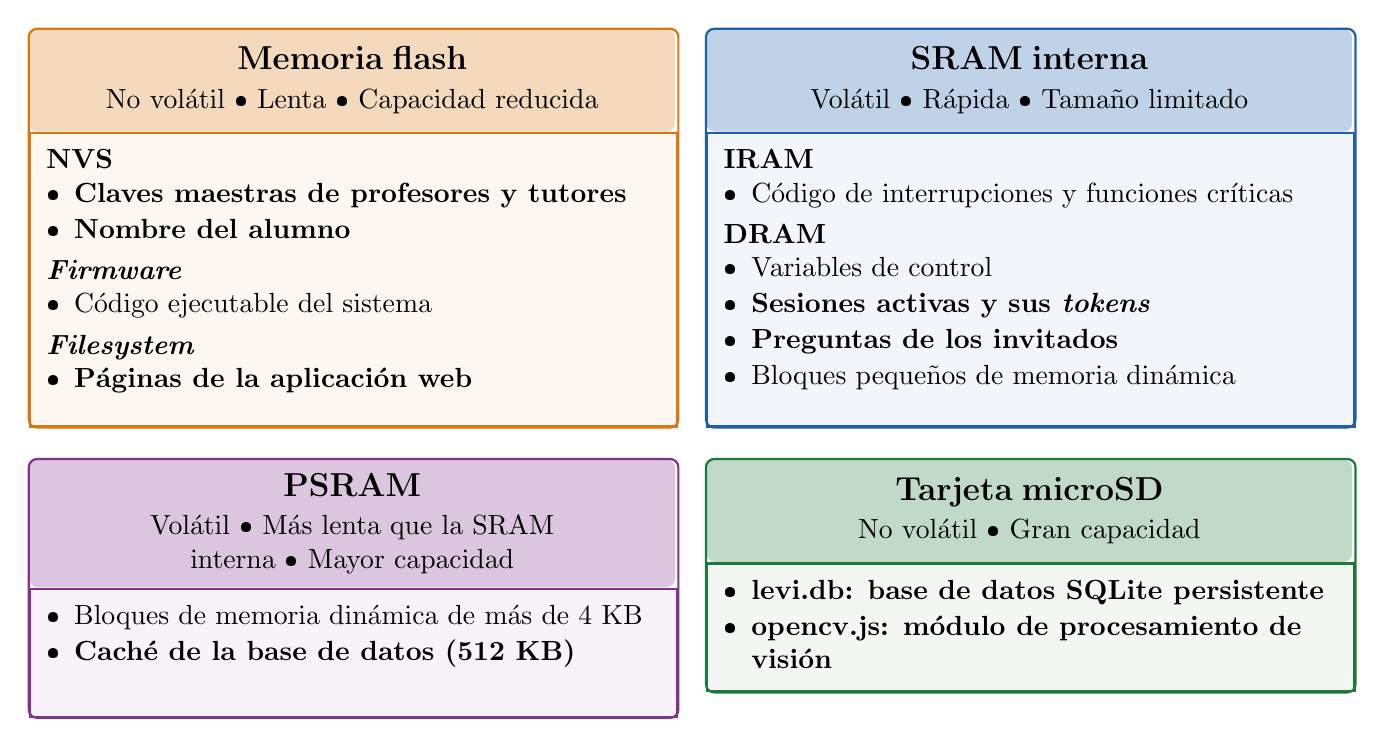
\begin{tikzpicture}

\bloque{f}{0,0}{cflash}{Memoria flash}{No volátil \textbullet{} Lenta \textbullet{} Capacidad reducida}{1.3cm}{3.3cm}{%
  \textbf{NVS}
  \lista{
    \item \textbf{Claves maestras de profesores y tutores}
    \item \textbf{Nombre del alumno}
  }
  \vspace{3pt}
  \textbf{\emph{Firmware}}
  \lista{
    \item Código ejecutable del sistema
  }
  \vspace{3pt}
  \textbf{\emph{Filesystem}}
  \lista{
    \item \textbf{Páginas de la aplicación web}
  }}

\bloque{s}{8.6,0}{csram}{SRAM interna}{Volátil \textbullet{} Rápida \textbullet{} Tamaño limitado}{1.3cm}{3.3cm}{%
  \textbf{IRAM}
  \lista{
    \item Código de interrupciones y funciones críticas
  }
  \vspace{3pt}
  \textbf{DRAM}
  \lista{
    \item Variables de control
    \item \textbf{Sesiones activas y sus \emph{tokens}}
    \item \textbf{Preguntas de los invitados}
    \item Bloques pequeños de memoria dinámica
  }}

\bloque{p}{$(fb.south west)+(0,-0.4)$}{cpsram}{PSRAM}{Volátil \textbullet{} Más lenta que la SRAM interna \textbullet{} Mayor capacidad}{1.3cm}{1.2cm}{%
  \lista{
    \item Bloques de memoria dinámica de más de 4 KB
    \item \textbf{Caché de la base de datos (512 KB)}
  }}

\bloque{m}{$(sb.south west)+(0,-0.4)$}{csd}{Tarjeta microSD}{No volátil \textbullet{} Gran capacidad}{1.3cm}{1.2cm}{%
  \lista{
    \item \textbf{levi.db: base de datos SQLite persistente}
    \item \textbf{opencv.js: módulo de procesamiento de visión}
  }}

\end{tikzpicture}
\end{document}
